%! TEX root = ../main.tex
\section{The double-beta decay}\label{sec:theory}
In this section we briefly review the theory of double-beta decay in its two most studied modes, the two-neutrino and the neutrinoless one, together with the mode which is relevant to this work, the Lorentz-violating one. We calculate the differential decay rates associated to the two-neutrino and the Lorentz-violating modes that will be cited in the following sections. Finally the current experimental knowledge about the Lorentz-violating mode is presented.
\subsection*{The two-neutrino double-beta decay}
\addcontentsline{toc}{subsection}{The two-neutrino double-beta decay}
The two-neutrino double-beta decay ($2\nbb$) processes, first suggested by M.~Goeppert-Mayer in 1935 \cite{PhysRev.48.512}, can be schematically defined as:
\[\begin{array}{lrl}
		\mathcal{N}(A,Z)\longrightarrow \mathcal{N}(A,Z+2)+2e^-+2\bar{\nu}_e & \qquad [2\nu\beta^-\beta^-] & \\
		\mathcal{N}(A,Z)\longrightarrow \mathcal{N}(A,Z-2)+2e^++2\nu_e & \qquad [2\nu\beta^+\beta^+] & ,\\
\end{array}\]
where $\mathcal{N}(A,Z)$ represents a nucleus with mass number $A$ and atomic number $Z$. A $2\nu\beta^-\beta^-$ ($2\nu\beta^+\beta^+$) process consists of the simultaneous $\beta^-$ ($\beta^+$) decay of two neutrons (protons) in the same nucleus. The processes are generated at second-order in the perturbative expansion of weak interactions in the Standard Model. The Feynman graph for $2\nu\beta^-\beta^-$ is shown in Fig.~\ref{fig:nbbfey}, left.
\begin{figure}[b]
	\centering%
	\makebox[\textwidth]{%
		\includegraphics[width=0.5\textwidth]{img/2nbbfey}%
		\includegraphics[width=0.5\textwidth]{img/0nbbfey}%
	}%
	\caption{Feynman graphs for two-neutrino (left) and neutrinoless (right) double-beta decay.}
	\label{fig:nbbfey}
\end{figure}

Since the $2\nbb$ decays have a four-body leptonic final state, the sum of the kinetic energies of the two decay electrons have a continuous spectrum from zero to the Q-value of the decay process (the recoil energy of the final nucleus is negligible), which is given by
\begin{equation}Q_{\beta\beta}=M_i-M_f-2m_e\;,\end{equation}
where $M_i$ and $M_f$ are, respectively, the masses of the initial and final nuclei (i.e. the energy levels of their ground states; if the transition occurs into an excited energy level of the final nucleus, $M_f$ must be replaced with the appropriate energy).

A nucleus $\mathcal{N}(A,Z)$ can decay through a $2\nbb$ process if its ground state has an energy which is larger than the ground-state energy of the nucleus $\mathcal{N}(A,Z\pm2)$ plus twice the electron mass. Moreover, if a nucleus can decay through both the $\beta$ and $2\nbb$ processes, in practice the latter is not observable, because its $\beta$ decay lifetime is much shorter than its $2\nbb$ decay lifetime (the half-life of $2\nbb$ is typically around $10^{19}-10^{24}$ yrs). Therefore, in practice the $2\nbb$ decay of a nucleus is observable only if its $\beta$ decay is energetically forbidden or strongly suppressed because of a large change of spin. The $\beta^-$ decay of a nucleus $\mathcal{N}(A,Z)$ is energetically forbidden if its ground-state energy is lower than the ground-state energy of the nucleus $\mathcal{N}(A,Z+1)$ plus the electron mass ($Q_{\beta^{-}}<0$). Typically, in $2\nu\beta^-\beta^-$ decays the energy levels of the three nuclei $\mathcal{N}(A,Z)$, $\mathcal{N}(A,Z+1)$, and $\mathcal{N}(A,Z+2)$ are of the type depicted in Fig.~\ref{fig:levelsGe76}, left, where the specific case of \ce{^{76}Ge}, \ce{^{76}As}, and \ce{^{76}Se} nuclei is considered.
\begin{figure}
	\centering
	\makebox[\textwidth]{%
		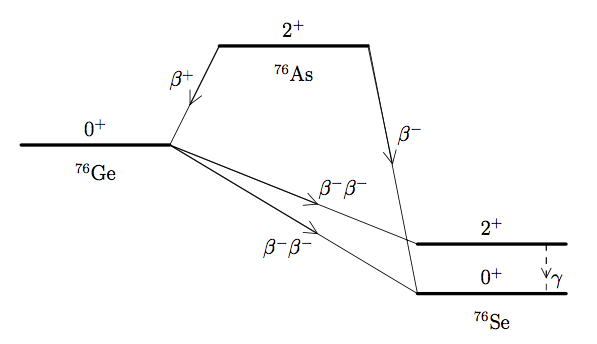
\includegraphics[width=0.5\textwidth]{img/levelsGe76}%
		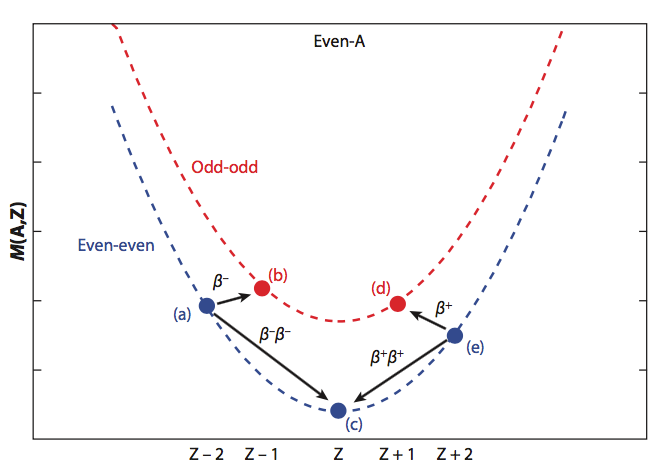
\includegraphics[width=0.5\textwidth]{img/masspar}%
	}%
	\caption{On the left: schematic illustration of the energy level structure of the $2\nu\beta^-\beta^-$ decay of \ce{^{76}Ge} into \ce{^{76}Se}. On the right: general energy level configuration for double-beta decay emitters. The situation for a nucleus with even mass number $A$ is presented: the mass parabola, representing the dependence of the binding energy $M(A,Z)$ on the atomic number $Z$, is plotted for even-even (even number of protons and neutrons) and odd-odd nuclei with the relevant $\beta$ and $\beta\beta$ decays among them.}
	\label{fig:levelsGe76}
\end{figure}

\marginnote{$2\nu\beta^-\beta^-$} The naturally occurring isotopes which can decay through the $2\nu\beta^-\beta^-$ process, with forbidden or suppressed $\beta^-$ decay are 35, and they are listed in \cite{Giunti:2007ry}. All of the initial and final nuclei in the $2\nu\beta^-\beta^-$ process are even-even, i.e.~they have an even number of protons and neutrons. Their binding energy is larger than the intermediate odd-odd nuclei one because of the pairing force acting between identical nucleons (see Fig.~\ref{fig:levelsGe76}, right). For the same reason, all of the initial and final nuclei have a $0^+$ ground state. Therefore, all ground-state to ground-state transitions are $0^+\rightarrow0^+$. Ground-state transitions to an excited state of the final nucleus may be energetically allowed, as in the case of the $\ce{^{76}Ge}\rightarrow\ce{^{76}Se}$ decay in Fig.~\ref{fig:levelsGe76}, left, in which there is an accessible $2^+$ excited state of \ce{^{76}Se}. However, due to a cancellation occurring in the phase space integral and the lower Q-value \cite{Tomoda:1991}, the $0^+\rightarrow2^+$ double-beta decay is suppressed with respect to $0^+\rightarrow0^+$.

\marginnote{$2\nu\beta^+\beta^+$} There are only six naturally occurring isotopes which can decay through the $2\nu\beta^+\beta^+$ process \cite{Haxton:1985am}. These isotopes have small Q-values and lifetimes which are much longer than the lifetimes of the $2\nu\beta^-\beta^-$. The reason for the rarity of $2\nu\beta^+\beta^+$-decaying isotopes and their small Q-values can be understood considering that the decay $\mathcal{N}(A,Z)\rightarrow\mathcal{N}(A,Z-1)$ can occur in two ways:
\[
	\begin{array}{lrl}
		\mathcal{N}(A,Z)\rightarrow\mathcal{N}(A,Z-1)+e^++\nu_e & \qquad [\beta^+] & \\
		e^-+\mathcal{N}(A,Z)\rightarrow\mathcal{N}(A,Z-1)+\nu_e & \qquad [\text{EC}]&. \\
	\end{array}
\]
Since $Q_\text{EC} = Q_{\beta^+}+2m_e$, the electron-capture process (EC) can occur even if the $\beta^+$ process is energetically forbidden ($Q_{\beta^+}<0$). Thus, in order to have an energetically forbidden $\mathcal{N}(A,Z)\rightarrow\mathcal{N}(A,Z-1)$ transitions, the ground-state energy of $\mathcal{N}(A,Z)$ must be smaller than the ground-state energy of the nucleus $\mathcal{N}(A,Z-1)$ minus the electron mass ($Q_\text{EC}<0$). Considering as a reference the energy of the ground-state energy of the intermediate nucleus, the ground-state energy of the initial nucleus in a $2\nu\beta^+\beta^+$ decay must be at least $2m_e$ lower than in the case of a $2\nu\beta^-\beta^-$ decay. This implies that $2\nu\beta^+\beta^+$-decaying isotopes are more rare than $2\nu\beta^-\beta^-$-decaying isotopes. Moreover, for the same energy difference between the ground states of the intermediate and final nuclei, the energy difference between the ground states of the initial and final nucleus in a $2\nu\beta^+\beta^+$ decay is at least $2m_e$ lower than in the case of a $2\nu\beta^-\beta^-$ decay, leading to a correspondingly smaller Q-value. For these reasons, $2\nu\beta^+\beta^+$ decay has been less studied than $2\nu\beta^-\beta^-$ decay and in the following we will consider only $2\nu\beta^-\beta^-$ decays (from now on we will simply refer to them with $2\nbb$). Let us only mention that $\mathcal{N}(A,Z)\rightarrow\mathcal{N}(A,Z-2)$ transitions can occur not only through $2\nu\beta^+\beta^+$ processes, but also through the processes 
\[
	\begin{array}{lrl}
		e^-+\mathcal{N}(A,Z)\rightarrow\mathcal{N}(A,Z-2)+e^++2\nu_e & \qquad [\text{EC}\beta^+] & \\
		2e^-+\mathcal{N}(A,Z)\rightarrow\mathcal{N}(A,Z-2)+2\nu_e & \qquad [2\text{EC}2\nu] & . \\
	\end{array}
\]

\marginnote{decay\\rate} The rate of $2\nbb$ can be calculated by invoking the recipe of the Fermi golden rule for simple $\beta$ decay. To a good approximation, the kinematic part (the phase space of the leptons emitted in the decay) and the nuclear part (the matrix element responsible for the transition probability between two nuclear states) can be factorized as
\begin{equation}\Gamma^{2\nu}=G^{2\nu}(Q_{\beta\beta},Z)|\mathcal{M}^{2\nu}|^2\;,\end{equation}
where $G^{2\nu}$ is obtained by integration over the phase space of four leptons emitted in the decay and can be calculated exactly. The nuclear matrix element $\mathcal{M}^{2\nu}$ deals with the nuclear structure of the transition and is much more difficult to evaluate.

Denoting the 4-momentum of the two electrons and the two anti-neutrinos by $p^\alpha_i=(E_i,\mathbf{p}_i)$ and $q^\alpha_i=(\omega_i,\mathbf{q}_i)$, respectively ($i=1,2$), the relevant matrix element is given by
\begin{equation}i\mathcal{M}=iG^2_FV^2_{ud}[\bar{u}(p_1)\gamma^\mu(1-\gamma_5)v(q_1)][\bar{u}(p_2)\gamma^\nu(1-\gamma_5)v(q_2)]J_{\mu\nu}-(p_1\leftrightarrow p_2)\;.\end{equation}
The hadronic tensor $J_{\mu\nu}$ corresponds to the product of two nuclear currents written in the impulse approximation \cite{Tomoda:1991}. Including the implementation of the long-wave and closure approximation fot the hadronic tensor \cite{Tomoda:1991}, we obtain
\begin{equation}\sum_\text{spin}|\mathcal{M}|^2=64G^4_F|V_{ud}|^4g^4_A(p_1\cdot p_2)(q_1\cdot q_2)|\mathcal{M}^{2\nu}|^2\;,\end{equation}
where the nuclear matrix element involves vector and axial couplings for Fermi and Gamow-Teller transitions in the form
\begin{equation}g^2_A\mathcal{M}^{2\nu}=g^2_V\mathcal{M}^{2\nu}_F-g^2_A\mathcal{M}^{2\nu}_{GT}\;.\end{equation}

General methods for phase-space factor calculations in double-beta decay have been developed \cite{Doi:1981,Doi:1983,Tomoda:1991}. The decay rate is given by integrating over all possible energies and angles of the leptons emitted in the decay. For the two-neutrino mode, these leptons are the two electrons and the two anti-neutrinos:
\begin{equation}\begin{split}
	%G^{2\nu} \propto \int \text{d}^3p_1\text{d}^3p_2\text{d}^3q_1\text{d}^3q_2F(Z,E_1)F(Z,E_2)\delta(E_1+E_1+\omega_1+\omega_2-E_F+E_I)\;,
		\text{d}\Gamma=\frac{1}{4}\int & \frac{\text{d}^3p_1}{(2\pi)^32E_1}\frac{\text{d}^3p_2}{(2\pi)^32E_2}\frac{\text{d}^3q_1}{(2\pi)^32\omega_1}\frac{\text{d}^3q_2}{(2\pi)^32\omega_2} \\
									   & \times F(Z,E_1)F(Z,E_2)\sum|\mathcal{M}|^2 \\
									   & \times 2\pi\delta(E_1+E_2+\omega_1+\omega_2-E_F+E_I)\;, \\
\end{split}\end{equation}
where $F(Z,E)$ is the Fermi function that describes the Coulomb effect on the outgoing electrons and $E_I$, $E_F$ are the energies of the parent and the daughter nucleus, respectively.

In the Primakoff–Rosen approximation \cite{PrimakoffRosen} for the non-relativistic Coulomb correction, the sum spectrum of the electrons energies can be analytically calculated. After a suitable change of integration variables, defining the sum of kinetic energies $K=T_1+T_2$ for the two electrons and integrating over the remaining variables, we obtain
\begin{equation}\frac{\text{d}\Gamma}{\text{d}K}=\Lambda\cdot(K^5+10K^4+40K^3+60K^2+30K)(Q_{\beta\beta}-K)^5\;,\label{eq:spectstd}\end{equation}
where $K$ is written in units of the electron mass. The overall constant factor is given by
\begin{equation}\Lambda=\frac{G_F^4g_A^4|V_{ud}|^4F^2_\text{PR}(Z)m_e^{11}}{7200\pi^7}|\mathcal{M}^{2\nu}|^2\;,\end{equation}
with $F_\text{PR}(Z)=2\pi\alpha/Z(\-e^{-2\pi\alpha Z})$. The distribution for \ce{^{76}Ge} is plotted in Fig.~\ref{fig:energyspectra}.
\begin{figure}
	\centering
	\includegraphics{img/energyspectra}
	\caption{Energy spectra for different double-beta decay modes of \ce{^{76}Ge}: the two-neutrino mode (blue), the Lorentz violating mode (red), the neutrinoless mode (green).}
	\label{fig:energyspectra}
\end{figure}

\subsection*{The neutrinoless double-beta decay}
\addcontentsline{toc}{subsection}{The neutrinoless double-beta decay}
The neutrinoless double-beta decay processes ($0\nbb$) of the types
\[
	\begin{array}{lrl}
		\mathcal{N}(A,Z)\longrightarrow \mathcal{N}(A,Z+2)+2e^- & \qquad [0\nu\beta^-\beta^-] & \\
		\mathcal{N}(A,Z)\longrightarrow \mathcal{N}(A,Z-2)+2e^+ & \qquad [0\nu\beta^+\beta^+] & , \\
	\end{array}
\]
which have been proposed by W.~H.~Furry in 1939 \cite{PhysRev.56.1184}, are forbidden in the minimal Standard Model, where the neutrinos are massless, because the conservation of the total lepton number is violated by two units. Considering that today we know, from oscillations experiments, that neutrinos are instead massive particles, there are two ways to characterize them: they could be Dirac (as all the other fundamental particles) or Majorana particles. Being a Majorana particle, as first proposed by Ettore Majorana \cite{Majorana1932}, basically means do not distinguish between particle and anti-particle. $0\nbb$ decays, in the standard interpretation, are possible if neutrinos are massive Majorana particles, with the Feynman diagram in Fig.~\ref{fig:nbbfey}, right. In this case, no neutrinos are emitted during the process and the experimental signature is a Dirac-delta function at $Q_{\beta\beta}$ in the summed energy spectrum (Fig.~\ref{fig:energyspectra}). A nucleus which can decay through a $2\nbb$ process can also decay through a $0\nbb$ process, albeit with a different lifetime ($\gtrsim10^{25}$ yr). Also the other double-beta decay modes mentioned above have their neutrinoless analog. However, as reviewed in \cite{Rodejohann:2011mu}, it should be pointed out that there are many other well-motivated Particle Physics scenarios and frameworks that allow for $0\nbb$, treated as negligible contributions in the standard interpretation.

Considerable experimental efforts are being dedicated to the detection of $0\nbb$, as such experiments represent the only practical way of establishing the nature of neutrino mass and therefore of shedding light on the mechanism of the tiny (but non-zero) neutrino mass generation established by neutrino oscillation experiments.

\subsection*{The Lorentz violating two-neutrino double-beta decay}
\addcontentsline{toc}{subsection}{The Lorentz violating two-neutrino double-beta decay}
Since the Standard Model of Particle Physics is known to provide a successful description of most Physics at low energies, compared to the Planck scale $m_p\sim10^{19}$ GeV, any signal of new Physics must appear at low energies in the form of an effective quantum field theory containing the Standard Model. The general effective quantum field theory constructed from the latter and allowing for arbitrary coordinate-independent Lorentz violation is called the Standard Model Extension \cite{SME1997,SME1998}. As an effective field theory it provides a link to the Planck scale through operators of non-renormalizable dimension. The Lagrangian of the Standard Model Extension consists of the usual Standard Model Lagrangian supplemented by all possible terms that can be constructed with the existing fields and that introduce violations of Lorentz symmetry. The additional terms have the form of Lorentz-violating operators coupled to vector coefficients, and they could arise in a variety of ways.

All quantum field operators for Lorentz violation involved in the propagation of neutrinos have been classified and enumerated \cite{SMEneutrinos}. Most of these can be studied using neutrino oscillations, which compare the way different neutrinos propagate and provide interferometric sensitivity to energy differences between them. Some effects cannot be detected by neutrino oscillations because they are produced by ‘oscillation-free’ operators that change all neutrino energies equally. Most of these can instead be studied by comparing neutrino propagation to other species, such as time-of-flight experiments matching the group velocity of neutrinos with the photons' one. However, four oscillation-free operators leave unaffected the neutrino group velocity and so cannot be detected in this way. Instead, they must be accessed through physical processes that involve neutrino phase-space properties, such as particle decays. These operators are rare examples of \textit{countershaded} Lorentz violations \cite{SMEcountersh}: Relativity-violating effects that could be enormous compared to ones suppressed by the ratio $m_W/m_P$ and that nonetheless could have escaped detection to date. These could provide an interesting path for building models with viable Lorentz violation obviating the typical requirement of a heavy suppression factor.

The four countershaded neutrino operators are of renormalizable mass dimension $d = 3$, are odd under CPT, and are controlled by coefficients conventionally denoted with $(a^{(3)}_\text{of})_{jm}$ , where $j$, $m$ are angular-momentum quantum numbers with $j = 0,1$. Conservation of energy and momentum is assured by taking these four coefficients to be constant as usual for couplings beyond the Standard Model, so all Physics other than Lorentz and CPT violation is conventional. Dimensional arguments suggest these coefficients are likely to dominate at accessible energies and can be measured sensitively in low-energy processes.

The anti-neutrino phase space element $\text{d}^3q$ is modified by the presence of these new operators:
\begin{equation}\omega^2\text{d}\omega\text{d}\Omega \;\longmapsto\; f(\omega)\text{d}\omega\text{d}\Omega\;,\end{equation}
where the anti-neutrino function
\begin{equation}f(\omega)\simeq\omega^2-\frac{1}{2}m_\nu^2-2\omega\delta\omega\end{equation}
encodes the Lorentz-violating modifications
\begin{equation}\delta\omega=-\sum_{jm}e^{im\omega_\oplus T_\oplus}\mathcal{N}_{jm}(a_\text{of}^{(3)})_{jm}\end{equation}
arising from the modified anti-neutrino dispersion relation \cite{SMEneutrinos} $\omega=|\mathbf{q}|+m_\nu^2/|\mathbf{q}|+\delta\omega$. The sidereal time $T_\oplus$ controls the harmonic variation of the anti-neutrino function in the laboratory produced by the Earth sidereal rotation at frequency $\omega_\oplus\simeq 2\pi/(23\text{ h } 56\text{ min})$. The factors $\mathcal{N}_{jm}$ contain information about the direction of propagation of the anti-neutrinos, expressed relative to the canonical sun-centered frame of reference \cite{frameor1,frameor2}.

\marginnote{decay\\rate} Following the same procedure as in the conventional two-neutrino double-beta decay, we integrate over all orientation, which implies that only isotropic effects are observable and hence that the residual spectrum depends only on $\aof\equiv(a_\text{of}^{(3)})_{00}/\sqrt{4\pi}$. After a suitable change of integration variables and defining the sum of kinetic energies $K=T_1+T_2$ for the two electrons, we obtain the electron sum spectrum
\begin{equation}
	\begin{split}
	\frac{\text{d}\Gamma}{\text{d}K} =& \Lambda \cdot(K^5+10K^4+40K^3+60K^2+30K) \\
									  & \times[(Q_{\beta\beta}-K)^5+10\aof(Q_{\beta\beta}-K)^4]\;. \\
	\end{split}\label{eq:totwidth}
\end{equation}
The total decay rate can be therefore expressed as an addition of two separate rates through a perturbation:
\begin{equation}\Gamma=\Gamma_0+\delta\Gamma\;,\end{equation}
where the first term is (\ref{eq:spectstd}) and the second one contains all the new Lorentz-violating information. The two differential decay rates are depicted in Fig.~\ref{fig:energyspectra}.

\subsubsection*{Current limits on $\aof$}
Conservative constraints on the $(\mathring{a}^{(3)}_\text{of})_{00}$ coefficient have been placed using published results from the Troitsk and Mainz experiments studying the endpoint of the tritium beta decay energy spectrum \cite{Diaz:2013saa}. An outside analysis of data from the two experiments gives $|(\mathring{a}^{(3)}_\text{of})_{00}|<2\cdot10^{-8}$ GeV for both of them. Constraints on the values of $\aof$ have also been extracted from studies of threshold effects in pion and kaon decays \cite{SMEneutrinos}, yielding $\aof<1.9\cdot10^{-7}$ GeV as the best upper limit.

A constraint from double-beta decay studies has been posed by the EXO--200 collaboration in Ref.~\cite{exo200}. A profile Likelihood scan over the number of Lorentz-violating double beta decay integral counts added to the standard $2\nbb$ spectrum is used to obtain a limit at the 90\% C.L, which is $\aof<7.6\cdot10^{-6}$ GeV. This is the first search for this parameter that fully accounts for experimental backgrounds and detector-related systematic uncertainties.
